\documentclass{standalone}
\usepackage{amsmath}
\usepackage{amssymb}
\usepackage{tikz}
\usetikzlibrary{positioning,arrows.meta,decorations.pathreplacing}
\begin{document}
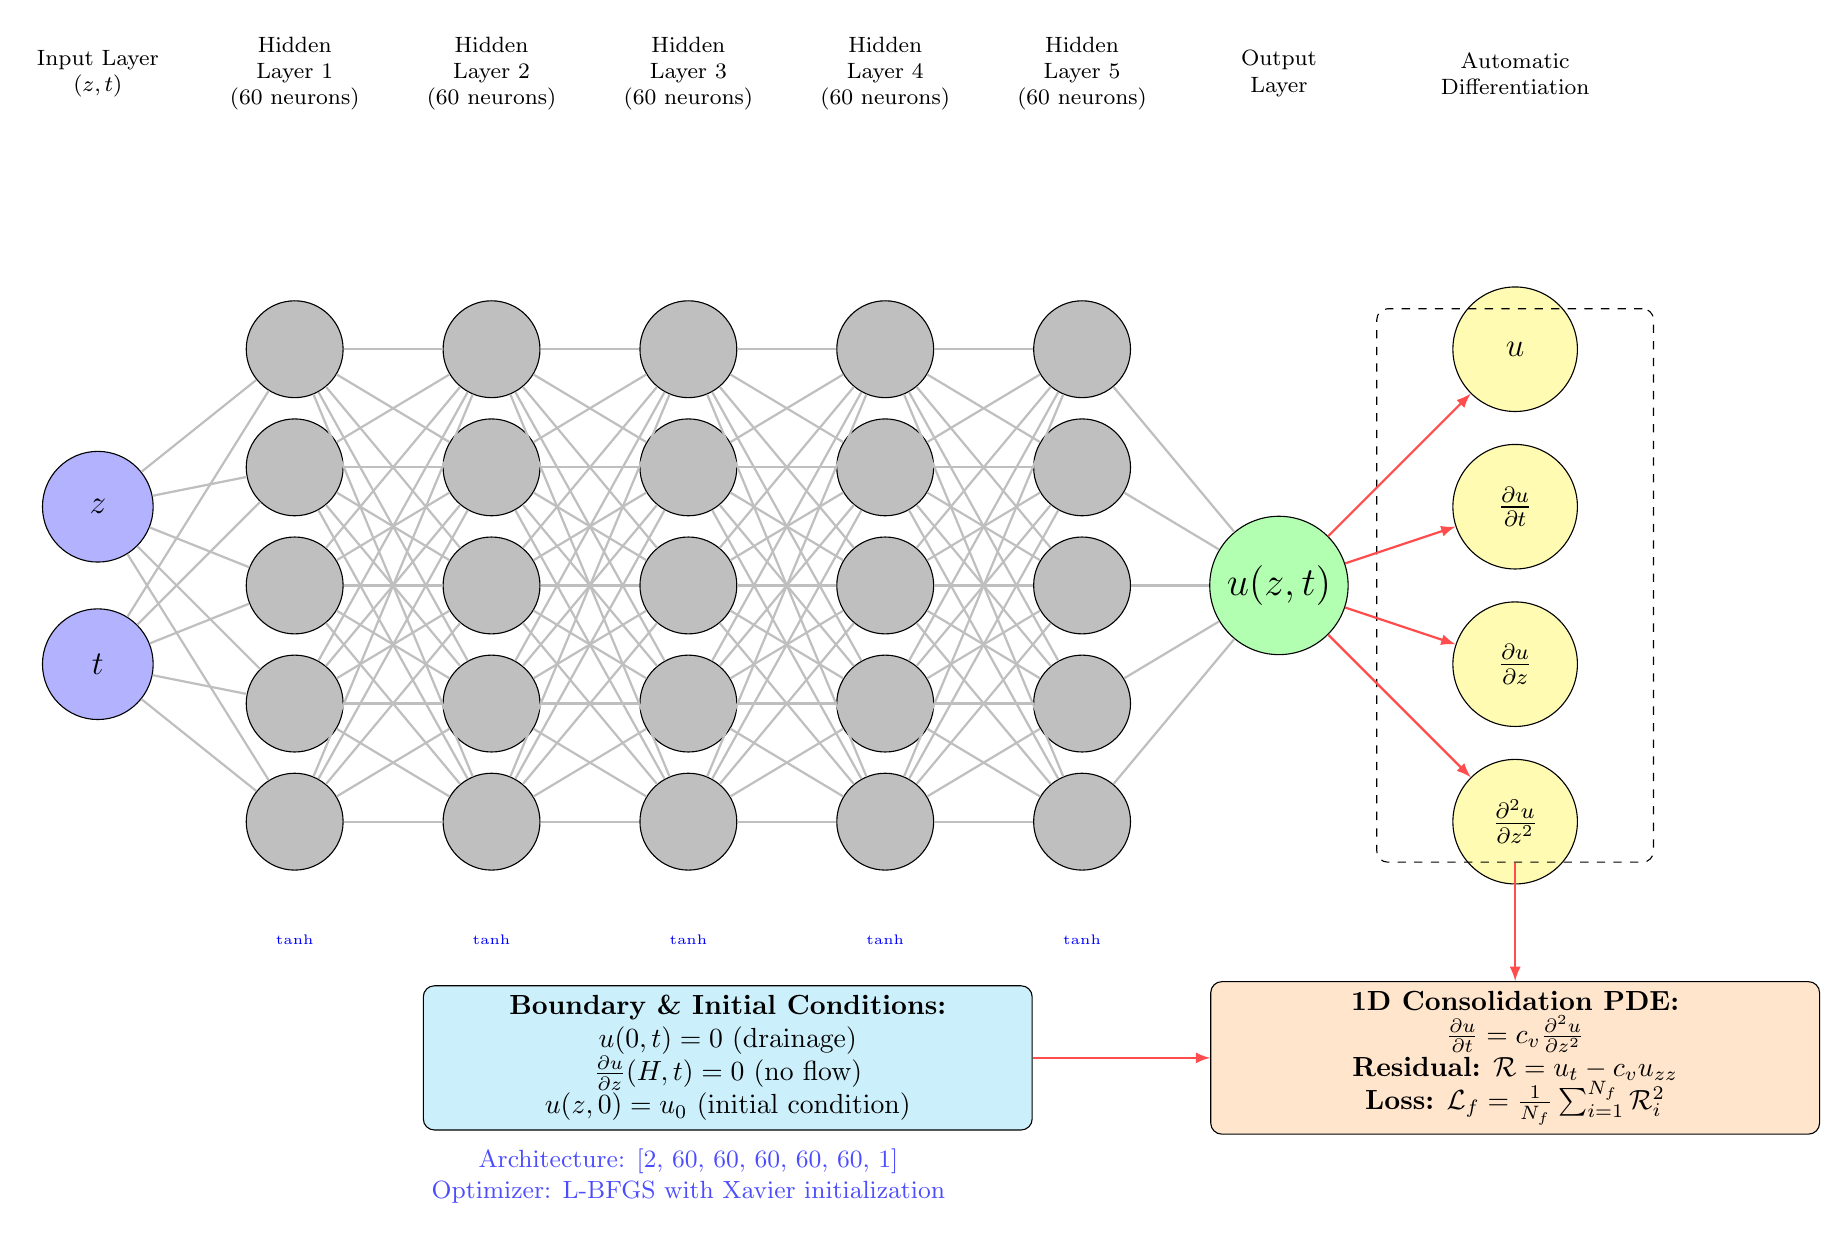
\begin{tikzpicture}[
    % Define styles for different types of nodes
    input/.style={circle, draw, fill=blue!30, minimum size=40pt, inner sep=0pt},
    hidden/.style={circle, draw, fill=gray!50, minimum size=35pt, inner sep=0pt},
    output/.style={circle, draw, fill=green!30, minimum size=50pt, inner sep=0pt},
    deriv/.style={circle, draw, fill=yellow!30, minimum size=45pt, inner sep=0pt},
    box/.style={rectangle, draw, dashed, rounded corners, minimum width=100pt, minimum height=200pt},
    pde/.style={rectangle, draw, fill=orange!20, minimum width=220pt, minimum height=50pt, rounded corners, align=center},
    conn/.style={gray!50, line width=0.8pt},
    arrow/.style={->, >=latex, thick, red!70},
    node_label/.style={font=\footnotesize, align=center}
]
    % Layer labels
    \node[node_label] at (0,6.5) {Input Layer\\$(z, t)$};
    \node[node_label] at (2.5,6.5) {Hidden\\Layer 1\\(60 neurons)};
    \node[node_label] at (5,6.5) {Hidden\\Layer 2\\(60 neurons)};
    \node[node_label] at (7.5,6.5) {Hidden\\Layer 3\\(60 neurons)};
    \node[node_label] at (10,6.5) {Hidden\\Layer 4\\(60 neurons)};
    \node[node_label] at (12.5,6.5) {Hidden\\Layer 5\\(60 neurons)};
    \node[node_label] at (15,6.5) {Output\\Layer};
    \node[node_label] at (18,6.5) {Automatic\\Differentiation};
    
    % Input layer
    \node[input] (z) at (0,1) {\large $z$};
    \node[input] (t) at (0,-1) {\large $t$};
    
    % Hidden layers (showing only 5 nodes per layer for clarity)
    \foreach \x [count=\layer] in {2.5,5,7.5,10,12.5} {
        \foreach \y [count=\i] in {3,1.5,0,-1.5,-3}
            \node[hidden] (h\layer-\i) at (\x,\y) {};
    }
    
    % Output layer
    \node[output] (u) at (15,0) {\Large $u(z,t)$};
    
    % Derivative nodes
    \node[deriv] (u_val) at (18,3) {\large $u$};
    \node[deriv] (u_t) at (18,1) {\large $\frac{\partial u}{\partial t}$};
    \node[deriv] (u_z) at (18,-1) {\large $\frac{\partial u}{\partial z}$};
    \node[deriv] (u_zz) at (18,-3) {\large $\frac{\partial^2 u}{\partial z^2}$};
    
    % Rectangle around derivative nodes
    \node[box] (deriv_box) at (18,0) {};
    
    % PDE loss box
    \node[pde] (pde) at (18,-6) {
        \textbf{1D Consolidation PDE:}\\
        $\frac{\partial u}{\partial t} = c_v \frac{\partial^2 u}{\partial z^2}$\\
        \textbf{Residual:} $\mathcal{R} = u_t - c_v u_{zz}$\\
        \textbf{Loss:} $\mathcal{L}_f = \frac{1}{N_f}\sum_{i=1}^{N_f} \mathcal{R}_i^2$
    };
    
    % Boundary conditions box
    \node[pde, fill=cyan!20] (bc) at (8,-6) {
        \textbf{Boundary \& Initial Conditions:}\\
        $u(0,t) = 0$ (drainage)\\
        $\frac{\partial u}{\partial z}(H,t) = 0$ (no flow)\\
        $u(z,0) = u_0$ (initial condition)
    };
    
    % Draw connections from inputs to first hidden layer
    \foreach \i in {1,...,5} {
        \draw[conn] (z) -- (h1-\i);
        \draw[conn] (t) -- (h1-\i);
    }
    
    % Connections between hidden layers (showing some connections)
    \foreach \layer in {1,...,4} {
        \pgfmathtruncatemacro{\nextlayer}{\layer+1}
        \foreach \i in {1,...,5}
            \foreach \j in {1,...,5}
                \draw[conn] (h\layer-\i) -- (h\nextlayer-\j);
    }
    
    % Last hidden layer to output
    \foreach \i in {1,...,5}
        \draw[conn] (h5-\i) -- (u);
    
    % Connections from u to derivative nodes
    \draw[arrow] (u) -- (u_val);
    \draw[arrow] (u) -- (u_t);
    \draw[arrow] (u) -- (u_z);
    \draw[arrow] (u) -- (u_zz);
    
    % Arrow from derivative box to PDE loss
    \draw[arrow] (deriv_box) -- (pde);
    
    % Arrow from boundary conditions
    \draw[arrow] (bc) -- (pde);
    
    % Add tanh activation labels
    \foreach \x in {2.5,5,7.5,10,12.5} {
        \node[font=\tiny, color=blue] at (\x, -4.5) {tanh};
    }
    
    % Add architecture annotation
    \node[font=\small, align=center, color=blue!70] at (7.5, -7.5) {
        Architecture: [2, 60, 60, 60, 60, 60, 1]\\
        Optimizer: L-BFGS with Xavier initialization
    };
    
\end{tikzpicture}
\end{document}